\documentclass[]{article}
\usepackage{lmodern}
\usepackage{amssymb,amsmath}
\usepackage{ifxetex,ifluatex}
\usepackage{fixltx2e} % provides \textsubscript
\ifnum 0\ifxetex 1\fi\ifluatex 1\fi=0 % if pdftex
  \usepackage[T1]{fontenc}
  \usepackage[utf8]{inputenc}
\else % if luatex or xelatex
  \ifxetex
    \usepackage{mathspec}
  \else
    \usepackage{fontspec}
  \fi
  \defaultfontfeatures{Ligatures=TeX,Scale=MatchLowercase}
\fi
% use upquote if available, for straight quotes in verbatim environments
\IfFileExists{upquote.sty}{\usepackage{upquote}}{}
% use microtype if available
\IfFileExists{microtype.sty}{%
\usepackage{microtype}
\UseMicrotypeSet[protrusion]{basicmath} % disable protrusion for tt fonts
}{}
\usepackage[margin=1in]{geometry}
\usepackage{hyperref}
\hypersetup{unicode=true,
            pdftitle={SM3\_Project},
            pdfauthor={Shingyan Kwong},
            pdfborder={0 0 0},
            breaklinks=true}
\urlstyle{same}  % don't use monospace font for urls
\usepackage{color}
\usepackage{fancyvrb}
\newcommand{\VerbBar}{|}
\newcommand{\VERB}{\Verb[commandchars=\\\{\}]}
\DefineVerbatimEnvironment{Highlighting}{Verbatim}{commandchars=\\\{\}}
% Add ',fontsize=\small' for more characters per line
\usepackage{framed}
\definecolor{shadecolor}{RGB}{248,248,248}
\newenvironment{Shaded}{\begin{snugshade}}{\end{snugshade}}
\newcommand{\KeywordTok}[1]{\textcolor[rgb]{0.13,0.29,0.53}{\textbf{#1}}}
\newcommand{\DataTypeTok}[1]{\textcolor[rgb]{0.13,0.29,0.53}{#1}}
\newcommand{\DecValTok}[1]{\textcolor[rgb]{0.00,0.00,0.81}{#1}}
\newcommand{\BaseNTok}[1]{\textcolor[rgb]{0.00,0.00,0.81}{#1}}
\newcommand{\FloatTok}[1]{\textcolor[rgb]{0.00,0.00,0.81}{#1}}
\newcommand{\ConstantTok}[1]{\textcolor[rgb]{0.00,0.00,0.00}{#1}}
\newcommand{\CharTok}[1]{\textcolor[rgb]{0.31,0.60,0.02}{#1}}
\newcommand{\SpecialCharTok}[1]{\textcolor[rgb]{0.00,0.00,0.00}{#1}}
\newcommand{\StringTok}[1]{\textcolor[rgb]{0.31,0.60,0.02}{#1}}
\newcommand{\VerbatimStringTok}[1]{\textcolor[rgb]{0.31,0.60,0.02}{#1}}
\newcommand{\SpecialStringTok}[1]{\textcolor[rgb]{0.31,0.60,0.02}{#1}}
\newcommand{\ImportTok}[1]{#1}
\newcommand{\CommentTok}[1]{\textcolor[rgb]{0.56,0.35,0.01}{\textit{#1}}}
\newcommand{\DocumentationTok}[1]{\textcolor[rgb]{0.56,0.35,0.01}{\textbf{\textit{#1}}}}
\newcommand{\AnnotationTok}[1]{\textcolor[rgb]{0.56,0.35,0.01}{\textbf{\textit{#1}}}}
\newcommand{\CommentVarTok}[1]{\textcolor[rgb]{0.56,0.35,0.01}{\textbf{\textit{#1}}}}
\newcommand{\OtherTok}[1]{\textcolor[rgb]{0.56,0.35,0.01}{#1}}
\newcommand{\FunctionTok}[1]{\textcolor[rgb]{0.00,0.00,0.00}{#1}}
\newcommand{\VariableTok}[1]{\textcolor[rgb]{0.00,0.00,0.00}{#1}}
\newcommand{\ControlFlowTok}[1]{\textcolor[rgb]{0.13,0.29,0.53}{\textbf{#1}}}
\newcommand{\OperatorTok}[1]{\textcolor[rgb]{0.81,0.36,0.00}{\textbf{#1}}}
\newcommand{\BuiltInTok}[1]{#1}
\newcommand{\ExtensionTok}[1]{#1}
\newcommand{\PreprocessorTok}[1]{\textcolor[rgb]{0.56,0.35,0.01}{\textit{#1}}}
\newcommand{\AttributeTok}[1]{\textcolor[rgb]{0.77,0.63,0.00}{#1}}
\newcommand{\RegionMarkerTok}[1]{#1}
\newcommand{\InformationTok}[1]{\textcolor[rgb]{0.56,0.35,0.01}{\textbf{\textit{#1}}}}
\newcommand{\WarningTok}[1]{\textcolor[rgb]{0.56,0.35,0.01}{\textbf{\textit{#1}}}}
\newcommand{\AlertTok}[1]{\textcolor[rgb]{0.94,0.16,0.16}{#1}}
\newcommand{\ErrorTok}[1]{\textcolor[rgb]{0.64,0.00,0.00}{\textbf{#1}}}
\newcommand{\NormalTok}[1]{#1}
\usepackage{graphicx,grffile}
\makeatletter
\def\maxwidth{\ifdim\Gin@nat@width>\linewidth\linewidth\else\Gin@nat@width\fi}
\def\maxheight{\ifdim\Gin@nat@height>\textheight\textheight\else\Gin@nat@height\fi}
\makeatother
% Scale images if necessary, so that they will not overflow the page
% margins by default, and it is still possible to overwrite the defaults
% using explicit options in \includegraphics[width, height, ...]{}
\setkeys{Gin}{width=\maxwidth,height=\maxheight,keepaspectratio}
\IfFileExists{parskip.sty}{%
\usepackage{parskip}
}{% else
\setlength{\parindent}{0pt}
\setlength{\parskip}{6pt plus 2pt minus 1pt}
}
\setlength{\emergencystretch}{3em}  % prevent overfull lines
\providecommand{\tightlist}{%
  \setlength{\itemsep}{0pt}\setlength{\parskip}{0pt}}
\setcounter{secnumdepth}{0}
% Redefines (sub)paragraphs to behave more like sections
\ifx\paragraph\undefined\else
\let\oldparagraph\paragraph
\renewcommand{\paragraph}[1]{\oldparagraph{#1}\mbox{}}
\fi
\ifx\subparagraph\undefined\else
\let\oldsubparagraph\subparagraph
\renewcommand{\subparagraph}[1]{\oldsubparagraph{#1}\mbox{}}
\fi

%%% Use protect on footnotes to avoid problems with footnotes in titles
\let\rmarkdownfootnote\footnote%
\def\footnote{\protect\rmarkdownfootnote}

%%% Change title format to be more compact
\usepackage{titling}

% Create subtitle command for use in maketitle
\newcommand{\subtitle}[1]{
  \posttitle{
    \begin{center}\large#1\end{center}
    }
}

\setlength{\droptitle}{-2em}
  \title{SM3\_Project}
  \pretitle{\vspace{\droptitle}\centering\huge}
  \posttitle{\par}
  \author{Shingyan Kwong}
  \preauthor{\centering\large\emph}
  \postauthor{\par}
  \predate{\centering\large\emph}
  \postdate{\par}
  \date{May 13, 2018}


\begin{document}
\maketitle

\section{Part A.}\label{part-a.}

\section{1.}\label{section}

\begin{Shaded}
\begin{Highlighting}[]
\KeywordTok{pairs}\NormalTok{(}\OperatorTok{~}\NormalTok{Height}\OperatorTok{+}\NormalTok{Weight}\OperatorTok{+}\NormalTok{Length,}\DataTypeTok{data=}\NormalTok{child)}
\end{Highlighting}
\end{Shaded}

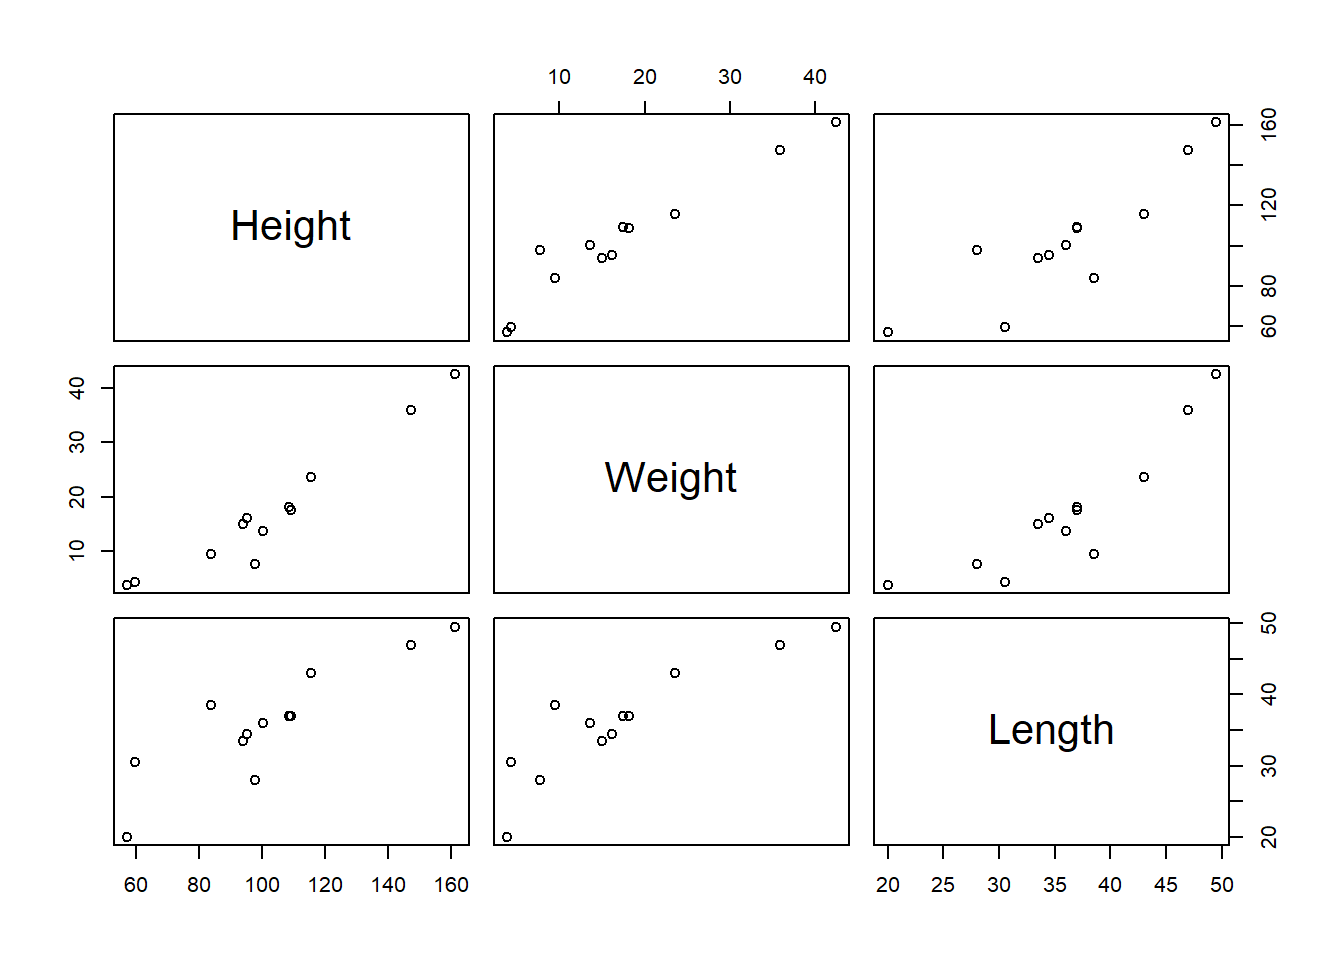
\includegraphics{project_files/figure-latex/unnamed-chunk-3-1.pdf}

There is evidence of a strong, positive linear relationship between
length and the two predictor variables, height and weight. The
associated correlation coefficients are 0.881 and 0.894 respectively.
There is also a strong, positive linear relationship between height and
weight. This suggests that the two predictors may be dependent one
another.

\section{2.}\label{section-1}

\begin{Shaded}
\begin{Highlighting}[]
\NormalTok{lm1<-}\KeywordTok{lm}\NormalTok{(Length}\OperatorTok{~}\NormalTok{Height}\OperatorTok{+}\NormalTok{Weight, }\DataTypeTok{data=}\NormalTok{child)}
\NormalTok{lm2<-}\KeywordTok{lm}\NormalTok{(Length}\OperatorTok{~}\NormalTok{Height, }\DataTypeTok{data=}\NormalTok{child)}
\NormalTok{lm3<-}\KeywordTok{lm}\NormalTok{(Length}\OperatorTok{~}\NormalTok{Weight, }\DataTypeTok{data=}\NormalTok{child)}
\end{Highlighting}
\end{Shaded}

\section{3.}\label{section-2}

The model assumptions which may be checked via diagnostic plots are as
follows.

Linearity: Check the residuals vs fitted and the residuals vs predictor
plots. Linearity is reasonable if random scatter above and below the 0
line is observed.

Constant Variance: Check scale location plot. Homoscedacity is
reasonable if constant variance of residuals is observed across the
scale location plot.

Normality: Check normal qq plot. Normality is reasonable if most points
between -2 and 2 are on/close to the diagonal line.

\section{4.}\label{section-3}

\section{Full model}\label{full-model}

\begin{Shaded}
\begin{Highlighting}[]
\KeywordTok{par}\NormalTok{(}\DataTypeTok{mfrow=}\KeywordTok{c}\NormalTok{(}\DecValTok{2}\NormalTok{,}\DecValTok{2}\NormalTok{))}
\KeywordTok{plot}\NormalTok{(lm1)}
\end{Highlighting}
\end{Shaded}

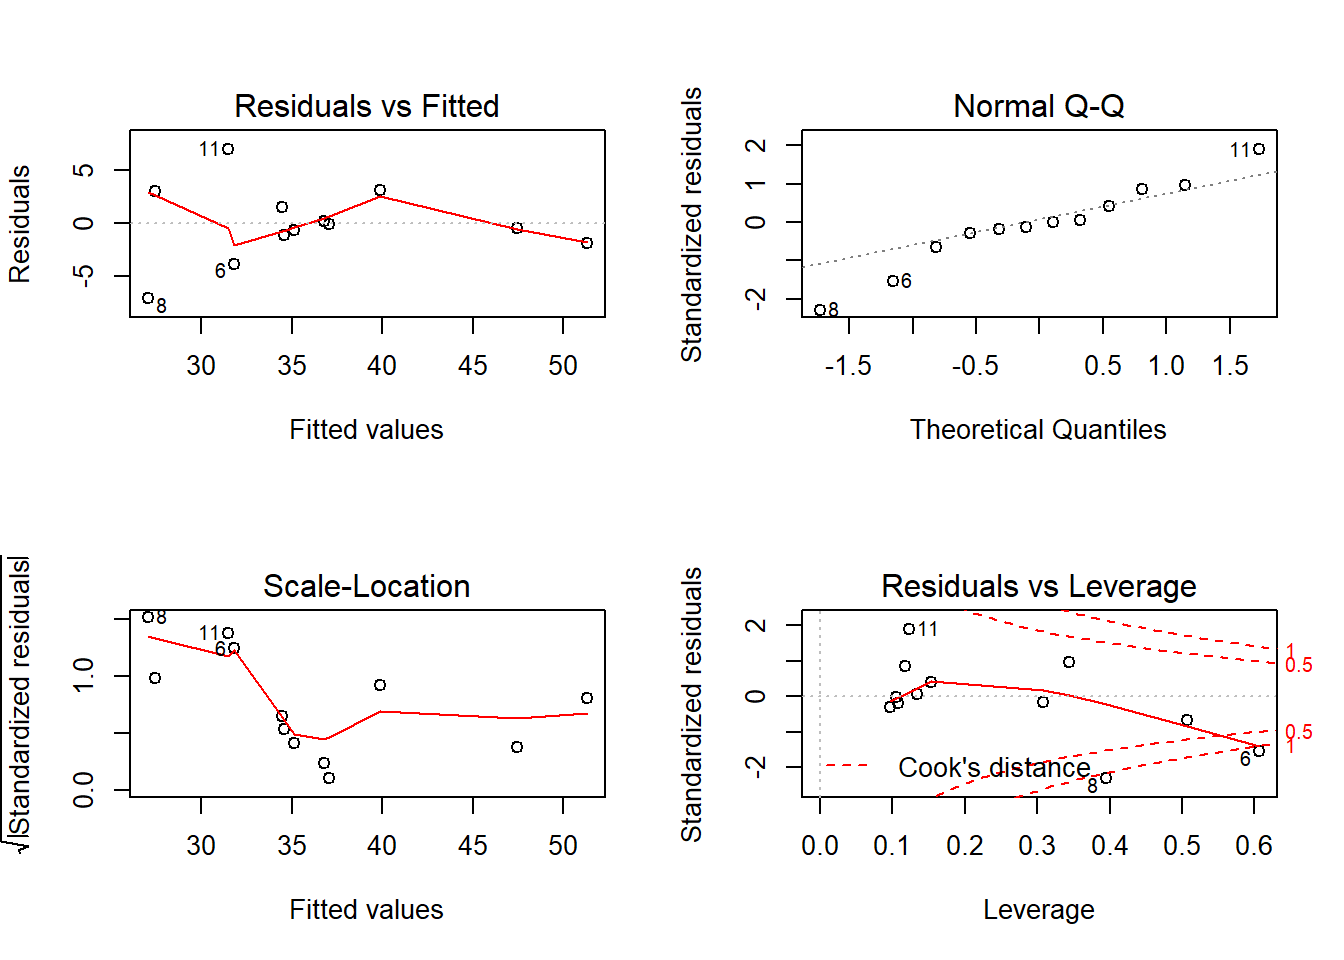
\includegraphics{project_files/figure-latex/unnamed-chunk-5-1.pdf}

\begin{Shaded}
\begin{Highlighting}[]
\KeywordTok{par}\NormalTok{(}\DataTypeTok{mfrow=}\KeywordTok{c}\NormalTok{(}\DecValTok{1}\NormalTok{,}\DecValTok{2}\NormalTok{))}
\NormalTok{res1<-}\KeywordTok{rstudent}\NormalTok{(lm1)}
\NormalTok{fit<-}\KeywordTok{fitted}\NormalTok{(lm1)}
\KeywordTok{plot}\NormalTok{(child}\OperatorTok{$}\NormalTok{Height,res1,}\DataTypeTok{main=}\StringTok{"Residuals vs height"}\NormalTok{,}\DataTypeTok{pch=}\DecValTok{20}\NormalTok{)}
\KeywordTok{abline}\NormalTok{(}\DecValTok{0}\NormalTok{,}\DecValTok{0}\NormalTok{,}\DataTypeTok{col=}\StringTok{"red"}\NormalTok{)}
\KeywordTok{plot}\NormalTok{(child}\OperatorTok{$}\NormalTok{Weight,res1,}\DataTypeTok{main=}\StringTok{"Residuals vs weight"}\NormalTok{,}\DataTypeTok{pch=}\DecValTok{20}\NormalTok{)}
\KeywordTok{abline}\NormalTok{(}\DecValTok{0}\NormalTok{,}\DecValTok{0}\NormalTok{,}\DataTypeTok{col=}\StringTok{"red"}\NormalTok{)}
\end{Highlighting}
\end{Shaded}

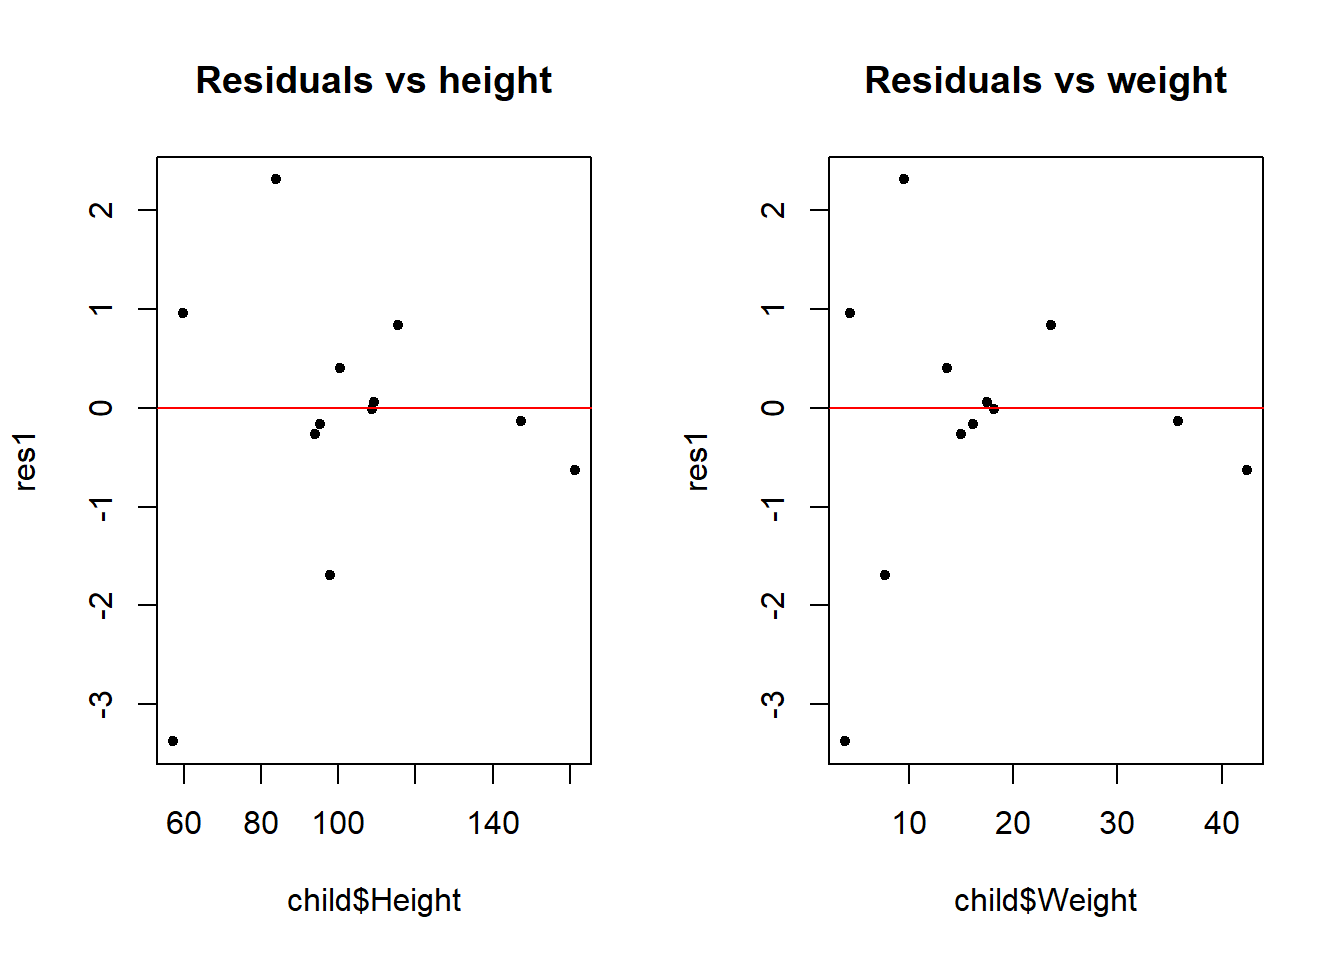
\includegraphics{project_files/figure-latex/unnamed-chunk-6-1.pdf}

Linearity: Given the small number of data points available, roughly
random scatter is observed in the residual vs fitted and residual vs
predictor plots. There is a couple of high residual points but it is not
too bad. Linearity is reasonable.

Constant variance: Scale location plots appear to show heteroscedacity.
Constant variance is not reasonable.

Normality: There is some minor departure from normality in the beginning
and the tails of the standardized residuals. Overall the points are
fairly close to the diagonal line. Normality is reasonable.

Leverage: There are 2 data points in the zone of danger. These high
leverage points are having a disproportionate effect on the model.

\section{Model with Weight only}\label{model-with-weight-only}

\begin{Shaded}
\begin{Highlighting}[]
\KeywordTok{par}\NormalTok{(}\DataTypeTok{mfrow=}\KeywordTok{c}\NormalTok{(}\DecValTok{2}\NormalTok{,}\DecValTok{2}\NormalTok{))}
\KeywordTok{plot}\NormalTok{(lm2)}
\end{Highlighting}
\end{Shaded}

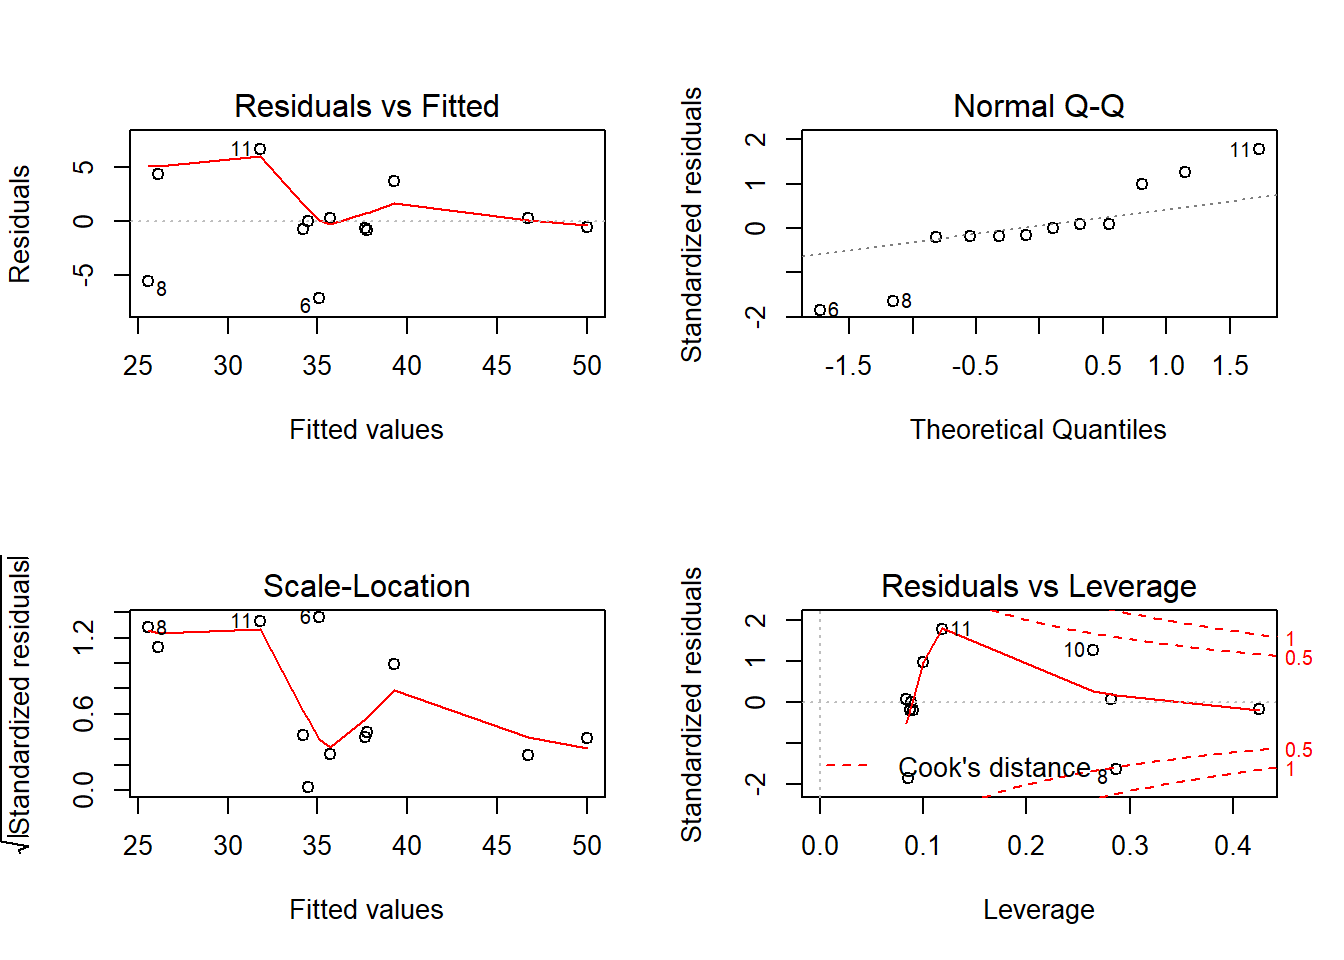
\includegraphics{project_files/figure-latex/unnamed-chunk-7-1.pdf}

\begin{Shaded}
\begin{Highlighting}[]
\KeywordTok{par}\NormalTok{(}\DataTypeTok{mfrow=}\KeywordTok{c}\NormalTok{(}\DecValTok{1}\NormalTok{,}\DecValTok{2}\NormalTok{))}
\NormalTok{res1<-}\KeywordTok{rstudent}\NormalTok{(lm2)}
\NormalTok{fit<-}\KeywordTok{fitted}\NormalTok{(lm2)}
\KeywordTok{plot}\NormalTok{(child}\OperatorTok{$}\NormalTok{Height,res1,}\DataTypeTok{main=}\StringTok{"Residuals vs height"}\NormalTok{,}\DataTypeTok{pch=}\DecValTok{20}\NormalTok{)}
\KeywordTok{abline}\NormalTok{(}\DecValTok{0}\NormalTok{,}\DecValTok{0}\NormalTok{,}\DataTypeTok{col=}\StringTok{"red"}\NormalTok{)}
\KeywordTok{plot}\NormalTok{(child}\OperatorTok{$}\NormalTok{Weight,res1,}\DataTypeTok{main=}\StringTok{"Residuals vs weight"}\NormalTok{,}\DataTypeTok{pch=}\DecValTok{20}\NormalTok{)}
\KeywordTok{abline}\NormalTok{(}\DecValTok{0}\NormalTok{,}\DecValTok{0}\NormalTok{,}\DataTypeTok{col=}\StringTok{"red"}\NormalTok{)}
\end{Highlighting}
\end{Shaded}

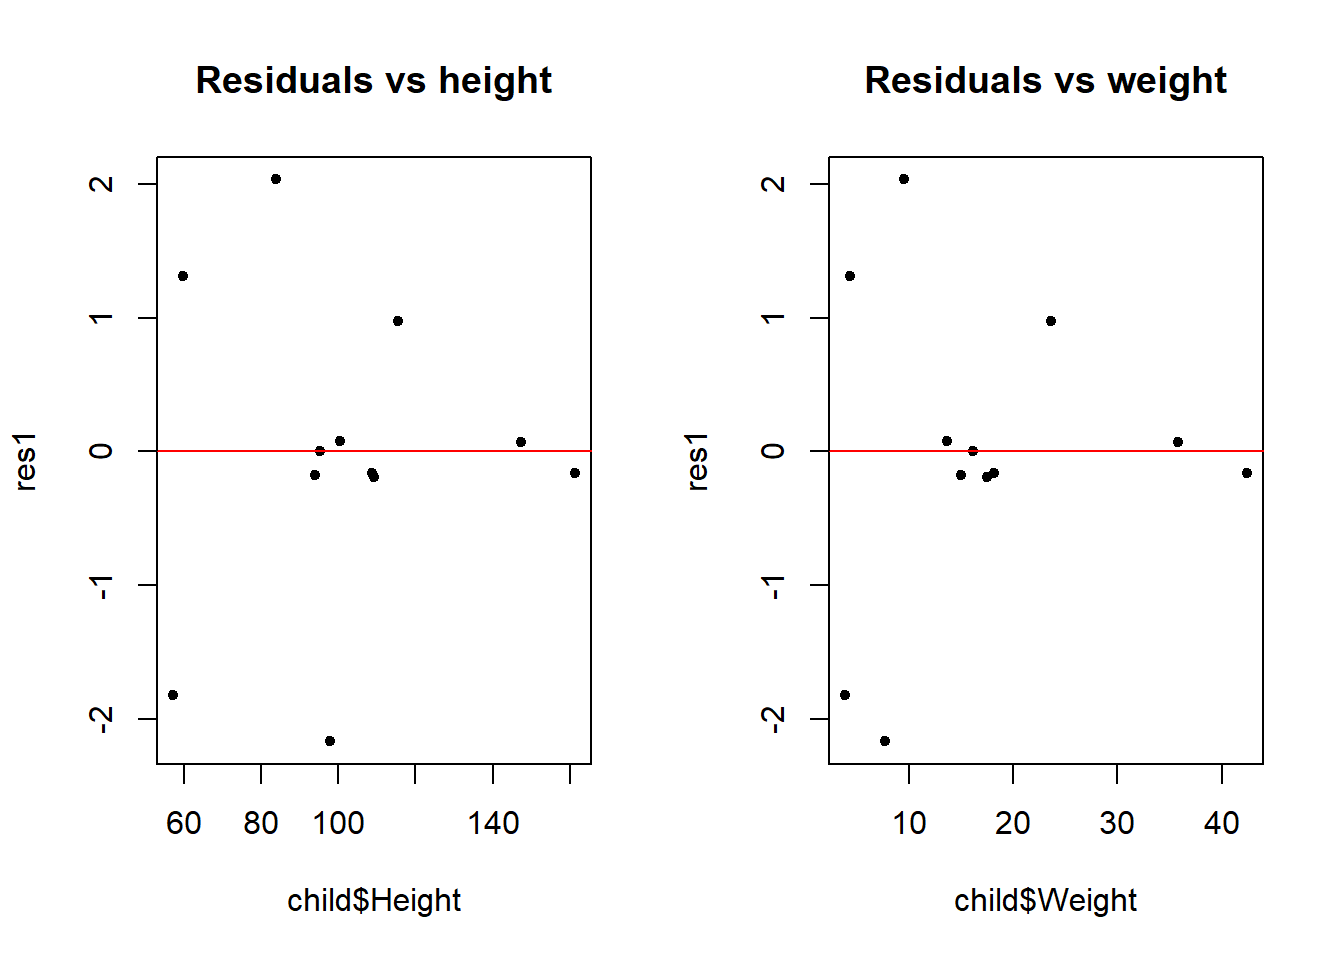
\includegraphics{project_files/figure-latex/unnamed-chunk-8-1.pdf}

Linearity: Non-random scatter observed in residual vs fitted and
residual vs predictor plots. Linearity is not reasonable.

Constant Variance: Variance appears to increase for the middle fitted
values and then decrease again. Constant variance is not reasonable.

Normality: There are several points deviating from the diagonal line on
the normal qq plot. Normality is not reasonable.

Leverage: There is one point with high leverage.

\section{Model with Height only}\label{model-with-height-only}

\begin{Shaded}
\begin{Highlighting}[]
\KeywordTok{par}\NormalTok{(}\DataTypeTok{mfrow=}\KeywordTok{c}\NormalTok{(}\DecValTok{2}\NormalTok{,}\DecValTok{2}\NormalTok{))}
\KeywordTok{plot}\NormalTok{(lm3)}
\end{Highlighting}
\end{Shaded}

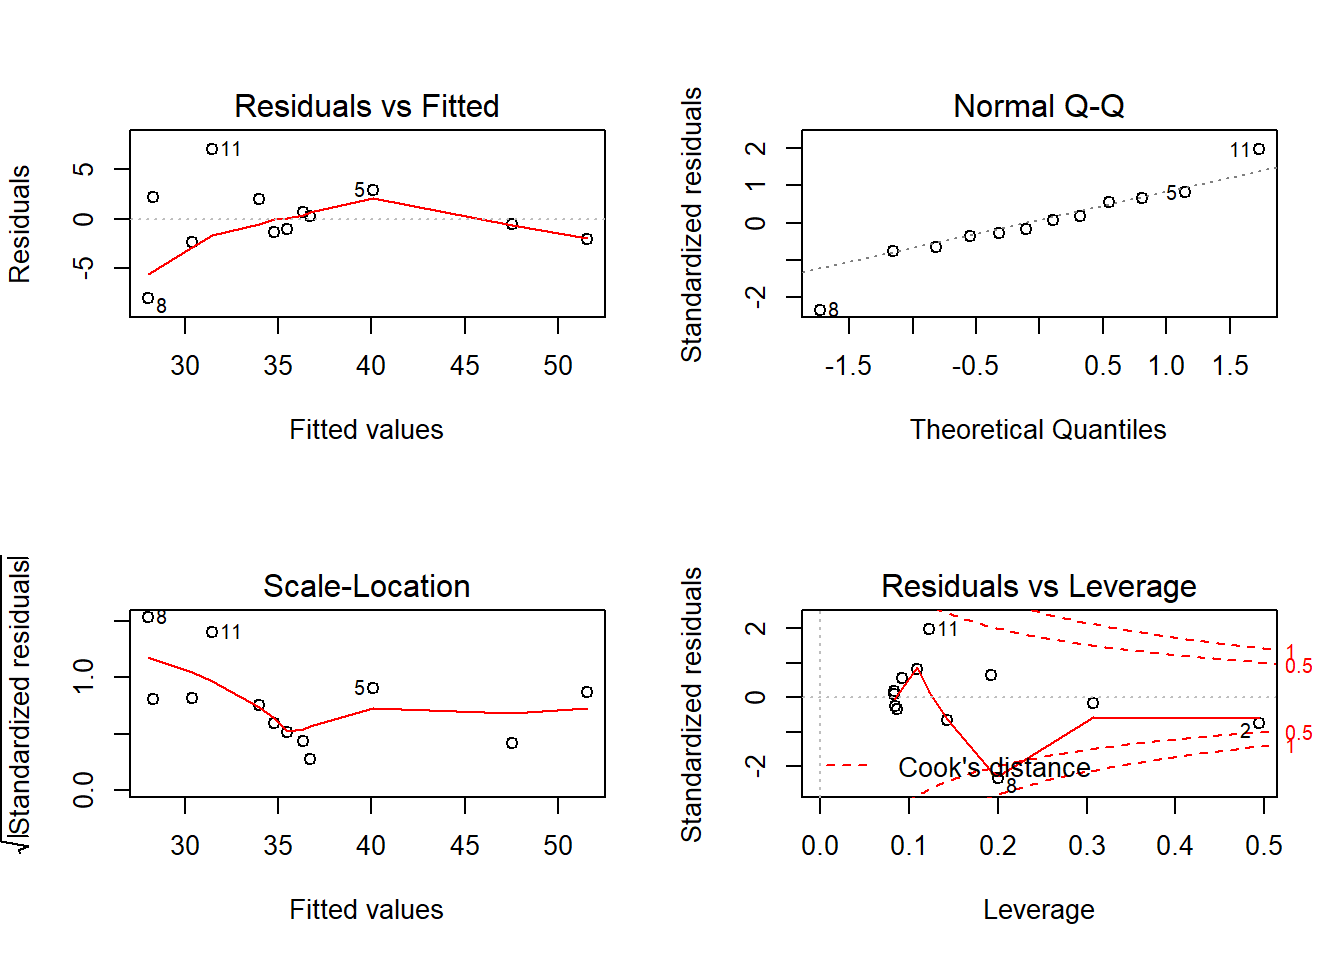
\includegraphics{project_files/figure-latex/unnamed-chunk-9-1.pdf}

\begin{Shaded}
\begin{Highlighting}[]
\KeywordTok{par}\NormalTok{(}\DataTypeTok{mfrow=}\KeywordTok{c}\NormalTok{(}\DecValTok{1}\NormalTok{,}\DecValTok{2}\NormalTok{))}
\NormalTok{res1<-}\KeywordTok{rstudent}\NormalTok{(lm3)}
\NormalTok{fit<-}\KeywordTok{fitted}\NormalTok{(lm3)}
\KeywordTok{plot}\NormalTok{(child}\OperatorTok{$}\NormalTok{Height,res1,}\DataTypeTok{main=}\StringTok{"Residuals vs height"}\NormalTok{,}\DataTypeTok{pch=}\DecValTok{20}\NormalTok{)}
\KeywordTok{abline}\NormalTok{(}\DecValTok{0}\NormalTok{,}\DecValTok{0}\NormalTok{,}\DataTypeTok{col=}\StringTok{"red"}\NormalTok{)}
\KeywordTok{plot}\NormalTok{(child}\OperatorTok{$}\NormalTok{Weight,res1,}\DataTypeTok{main=}\StringTok{"Residuals vs weight"}\NormalTok{,}\DataTypeTok{pch=}\DecValTok{20}\NormalTok{)}
\KeywordTok{abline}\NormalTok{(}\DecValTok{0}\NormalTok{,}\DecValTok{0}\NormalTok{,}\DataTypeTok{col=}\StringTok{"red"}\NormalTok{)}
\end{Highlighting}
\end{Shaded}

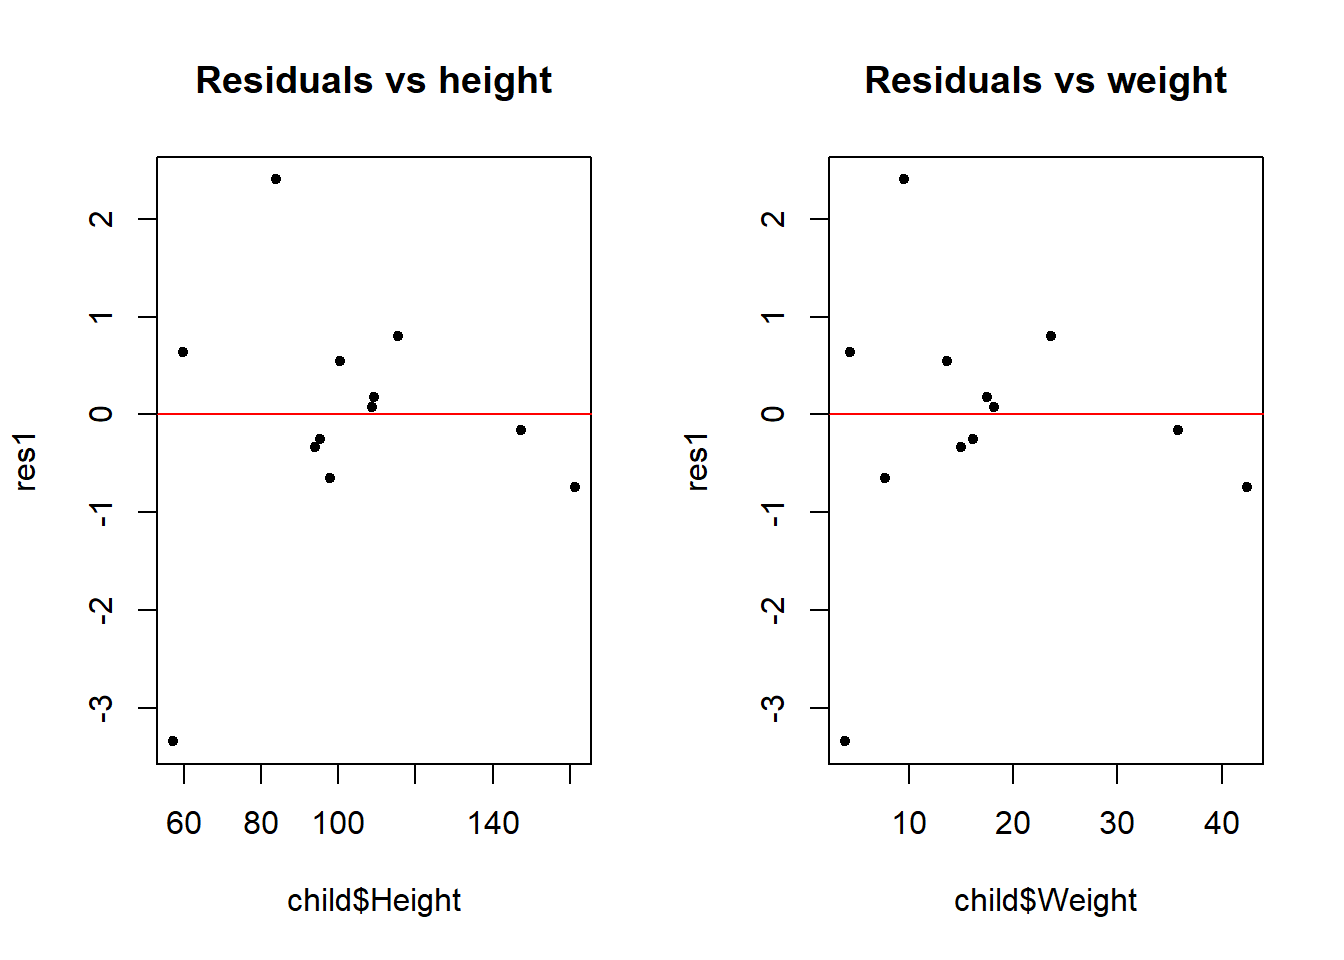
\includegraphics{project_files/figure-latex/unnamed-chunk-10-1.pdf}

Linearity: Rough random scatter in observed in residual vs fitted and
residual vs predictor plots. The fitted plot shows some evidence of
curvature but overall it is acceptable. Linearity is reasonable.

Constant Variance: Variance is roughly constant across the scale
location plot. Constant variance is reasonable.

Normality: Most points are close to the diagonal line except 2.
Normality is reasonable.

Leverage: There is one data point with high leverage.

\section{5. Comparison of the three
models}\label{comparison-of-the-three-models}

\begin{Shaded}
\begin{Highlighting}[]
\KeywordTok{summary}\NormalTok{(lm1)}
\end{Highlighting}
\end{Shaded}

\begin{verbatim}
## 
## Call:
## lm(formula = Length ~ Height + Weight, data = child)
## 
## Residuals:
##     Min      1Q  Median      3Q     Max 
## -7.0497 -1.2588 -0.2576  1.8987  7.0030 
## 
## Coefficients:
##             Estimate Std. Error t value Pr(>|t|)  
## (Intercept) 21.00828    8.74782   2.402   0.0398 *
## Height       0.07729    0.14192   0.545   0.5993  
## Weight       0.42081    0.36405   1.156   0.2775  
## ---
## Signif. codes:  0 '***' 0.001 '**' 0.01 '*' 0.05 '.' 0.1 ' ' 1
## 
## Residual standard error: 3.943 on 9 degrees of freedom
## Multiple R-squared:  0.8054, Adjusted R-squared:  0.7621 
## F-statistic: 18.62 on 2 and 9 DF,  p-value: 0.0006332
\end{verbatim}

\begin{Shaded}
\begin{Highlighting}[]
\KeywordTok{summary}\NormalTok{(lm2)}
\end{Highlighting}
\end{Shaded}

\begin{verbatim}
## 
## Call:
## lm(formula = Length ~ Height, data = child)
## 
## Residuals:
##     Min      1Q  Median      3Q     Max 
## -7.0996 -0.7246 -0.2608  1.1585  6.6826 
## 
## Coefficients:
##             Estimate Std. Error t value Pr(>|t|)    
## (Intercept) 12.12402    4.24711   2.855 0.017113 *  
## Height       0.23495    0.03986   5.894 0.000152 ***
## ---
## Signif. codes:  0 '***' 0.001 '**' 0.01 '*' 0.05 '.' 0.1 ' ' 1
## 
## Residual standard error: 4.008 on 10 degrees of freedom
## Multiple R-squared:  0.7765, Adjusted R-squared:  0.7541 
## F-statistic: 34.74 on 1 and 10 DF,  p-value: 0.0001523
\end{verbatim}

\begin{Shaded}
\begin{Highlighting}[]
\KeywordTok{summary}\NormalTok{(lm3)}
\end{Highlighting}
\end{Shaded}

\begin{verbatim}
## 
## Call:
## lm(formula = Length ~ Weight, data = child)
## 
## Residuals:
##     Min      1Q  Median      3Q     Max 
## -7.9958 -1.4818 -0.1334  2.0899  7.0378 
## 
## Coefficients:
##             Estimate Std. Error t value Pr(>|t|)    
## (Intercept) 25.63596    2.00425  12.791 1.60e-07 ***
## Weight       0.61136    0.09698   6.304 8.86e-05 ***
## ---
## Signif. codes:  0 '***' 0.001 '**' 0.01 '*' 0.05 '.' 0.1 ' ' 1
## 
## Residual standard error: 3.801 on 10 degrees of freedom
## Multiple R-squared:  0.7989, Adjusted R-squared:  0.7788 
## F-statistic: 39.74 on 1 and 10 DF,  p-value: 8.865e-05
\end{verbatim}

\begin{enumerate}
\def\labelenumi{(\alph{enumi})}
\item
\end{enumerate}

In the full model, neither predictor variables is statistically
significant (at the 0.05 level), and the numerical values of the two
coefficients are both smaller than those of the single predictor models.

\begin{enumerate}
\def\labelenumi{(\alph{enumi})}
\setcounter{enumi}{1}
\item
\end{enumerate}

Full model:

Holding height constant, the full model predicts that an increase of of
1kg will on average increase the length of the cathetar by 0.42081cm.

Weight only model:

Without regard for height, this model predicts that an increase of 1kg
will on average increase the cathetar length by 0.61136cm.

\section{6}\label{section-4}

\subsubsection{(a) We construct the model matrices for the height only
and weight only
models.}\label{a-we-construct-the-model-matrices-for-the-height-only-and-weight-only-models.}

\begin{verbatim}
##    (Intercept) Height
## 1            1 108.70
## 2            1 161.29
## 3            1  95.25
## 4            1 100.33
## 5            1 115.57
## 6            1  97.79
## 7            1 109.22
## 8            1  57.15
## 9            1  93.98
## 10           1  59.69
## 11           1  83.82
## 12           1 147.32
## attr(,"assign")
## [1] 0 1
\end{verbatim}

\begin{verbatim}
##    (Intercept) Weight
## 1            1  18.14
## 2            1  42.41
## 3            1  16.10
## 4            1  13.61
## 5            1  23.59
## 6            1   7.71
## 7            1  17.46
## 8            1   3.86
## 9            1  14.97
## 10           1   4.31
## 11           1   9.53
## 12           1  35.83
## attr(,"assign")
## [1] 0 1
\end{verbatim}

Here, we define \(\mathbf{1} := (1,1,1,1,1,1,1,1,1,1,1,1)\), the vector
of intercepts for both models. We also denote the vector of height
values by \(\mathbf{x}_1\) and the vector of weight values by
\(\mathbf{x}_2\). Then we find that:

\(\mathcal{L}_1\) is the space spanned by the columns of M2, that is
\(\mathcal{L}_1 = span \{ \mathbf{1}, \mathbf{x}_1 \}\)

\(\mathcal{L}_2\) is the space spanned by the columns of M3, that is
\(\mathcal{L}_2 = span \{ \mathbf{1}, \mathbf{x}_2 \}\)

Then, the intersection of the two subspaces is the intercept column,
that is \(\mathcal{L}_1 \cap \mathcal{L}_2 = span { \{\mathbf{1} \} }.\)

\subsubsection{(b)}\label{b}

We note that \((\mathcal{L}_1 \cap \mathcal{L}_2)^{\perp}\) is the
subspace of all vectors orthogonal to \(\mathbf{1}\). Then, in order to
find the intersections of \(\mathcal{L}_1\) and \(\mathcal{L}_2\) with
\((\mathcal{L}_1 \cap \mathcal{L}_2)^{\perp}\), we first find
orthonormal bases for \(\mathcal{L}_1\) and \(\mathcal{L}_2\).

We achive this by applying the Gram-Schmidt process. First, we define
the basis vectors for both subspaces, and a function norm\_vec to find
the norm of a vector:

\begin{Shaded}
\begin{Highlighting}[]
\NormalTok{one <-}\StringTok{ }\KeywordTok{c}\NormalTok{(}\DecValTok{1}\NormalTok{,}\DecValTok{1}\NormalTok{,}\DecValTok{1}\NormalTok{,}\DecValTok{1}\NormalTok{,}\DecValTok{1}\NormalTok{,}\DecValTok{1}\NormalTok{,}\DecValTok{1}\NormalTok{,}\DecValTok{1}\NormalTok{,}\DecValTok{1}\NormalTok{,}\DecValTok{1}\NormalTok{,}\DecValTok{1}\NormalTok{,}\DecValTok{1}\NormalTok{) }\CommentTok{# intercept vector}
\NormalTok{x1 <-}\StringTok{ }\NormalTok{M2[,}\DecValTok{2}\NormalTok{] }\CommentTok{# vector of height values}
\NormalTok{x2 <-}\StringTok{ }\NormalTok{M3[,}\DecValTok{2}\NormalTok{] }\CommentTok{# vector of weight values}
\NormalTok{norm_vec <-}\StringTok{ }\ControlFlowTok{function}\NormalTok{(x) }\KeywordTok{sqrt}\NormalTok{(}\KeywordTok{as.numeric}\NormalTok{(}\KeywordTok{t}\NormalTok{(x) }\OperatorTok\StringTok{ }\NormalTok{x))}
\end{Highlighting}
\end{Shaded}

Next, we find an orthonormal basis for \(\mathcal{L}_1\):

\begin{Shaded}
\begin{Highlighting}[]
\NormalTok{v1 <-}\StringTok{ }\NormalTok{one }\OperatorTok{/}\StringTok{ }\KeywordTok{norm_vec}\NormalTok{(one)}
\NormalTok{v2_ <-}\StringTok{ }\NormalTok{x1 }\OperatorTok{-}\StringTok{ }\KeywordTok{as.numeric}\NormalTok{((}\KeywordTok{t}\NormalTok{(x1) }\OperatorTok\StringTok{ }\NormalTok{v1)) }\OperatorTok{*}\StringTok{ }\NormalTok{v1}
\NormalTok{v2 <-}\StringTok{ }\NormalTok{v2_ }\OperatorTok{/}\StringTok{ }\KeywordTok{norm_vec}\NormalTok{(v2_)}
\end{Highlighting}
\end{Shaded}

Then \(\mathcal{L}_1 = span \{\mathbf{v}1, \mathbf{v}2\}\).

Now, an orthonormal basis for \(\mathcal{L}_2\):

\begin{Shaded}
\begin{Highlighting}[]
\NormalTok{w1 <-}\StringTok{ }\NormalTok{one }\OperatorTok{/}\StringTok{ }\KeywordTok{norm_vec}\NormalTok{(one)}
\NormalTok{w2_ <-}\StringTok{ }\NormalTok{x2 }\OperatorTok{-}\StringTok{ }\KeywordTok{as.numeric}\NormalTok{((}\KeywordTok{t}\NormalTok{(x2) }\OperatorTok\StringTok{ }\NormalTok{w1)) }\OperatorTok{*}\StringTok{ }\NormalTok{w1}
\NormalTok{w2 <-}\StringTok{ }\NormalTok{w2_ }\OperatorTok{/}\StringTok{ }\KeywordTok{norm_vec}\NormalTok{(w2_)}
\end{Highlighting}
\end{Shaded}

Then \(\mathcal{L}_2 = span \{\mathbf{w}1, \mathbf{w}2\}\).

Now, we have that \(\mathbf{v}_1 = \mathbf{w}_1\) is parallel to
\(\mathbf{1}\), and that \(\mathbf{v}_2\) and \(\mathbf{w}_2\) are
orthogonal to \(\mathbf{1}\), that is,
\(\mathbf{v}_2, \mathbf{w}_2 \in ({\mathcal{L}_1 \cap \mathcal{L}_2})^{\perp}\).

As a result, we find that:

\[ \mathcal{L}_1 \cap ({\mathcal{L}_1 \cap \mathcal{L}_2})^{\perp} = span \{ \mathbf{v}_2 \}; \]

\[ \mathcal{L}_2 \cap ({\mathcal{L}_1 \cap \mathcal{L}_2})^{\perp} = span \{ \mathbf{w}_2 \}. \]

\subsubsection{(c)}\label{c}

Given that both
\(\mathcal{L}_1 \cap ({\mathcal{L}_1 \cap \mathcal{L}_2})^{\perp}\) and
\(\mathcal{L}_2 \cap ({\mathcal{L}_1 \cap \mathcal{L}_2})^{\perp}\) are
one-dimensional subspace, we can compute the angle between them using
the relation:

\[
\cos \theta = \frac{ \langle \mathbf{u}, \mathbf{v} \rangle }{||\mathbf{u}|| \; ||\mathbf{v}||}
\]

Where \(\mathbf{u}\) and \(\mathbf{v}\) are two vectors and \(\theta\)
is the angle between them.

We compute the angle between the two spaces in \textbf{(b)} as follows:

\begin{Shaded}
\begin{Highlighting}[]
\NormalTok{dot <-}\StringTok{ }\KeywordTok{t}\NormalTok{(v2) }\OperatorTok\StringTok{ }\NormalTok{(w2)}
\NormalTok{norm_v2 <-}\StringTok{ }\KeywordTok{norm_vec}\NormalTok{(v2)}
\NormalTok{norm_w2 <-}\StringTok{ }\KeywordTok{norm_vec}\NormalTok{(w2)}
\NormalTok{theta <-}\StringTok{ }\KeywordTok{acos}\NormalTok{(dot}\OperatorTok{/}\NormalTok{(norm_v2 }\OperatorTok{*}\StringTok{ }\NormalTok{norm_w2))}
\NormalTok{theta}
\end{Highlighting}
\end{Shaded}

\begin{verbatim}
##           [,1]
## [1,] 0.2799352
\end{verbatim}

The angle is not \(\pi\) indicating that the two spaces are not
orthogonal. This suggests that height and weight are not independent. In
fact they are fairly correlated.

\section{7}\label{section-5}

Picking a model.

\begin{center}\rule{0.5\linewidth}{\linethickness}\end{center}

Comparing these three models, lm3 (length\textasciitilde{}weight) is
better than others. From the analysis of diagnostic plots of these three
models, the four assumptions in lm3 can be considered as the most
reasonable. Moreover, the angle between two spaces is approximately
equal to two, which means they are not orthogonal to each other.
Furthermore, there exists linear relationship between the two predictor
variables (height and weight) with correlation 0.961. Overall, weight as
the predictor variable and length as the response variables is the most
appropriate model.

\begin{center}\rule{0.5\linewidth}{\linethickness}\end{center}

\section{Part B}\label{part-b}

\subsection{Introduction}\label{introduction}

In this section we obtain a predictive model for mammographic mass
severity, a measure of the status of mammographic mass lesions, on a
scale from 0 to 1, where 0 is assigned to a benign tumor, and 1 is
assigned to a malignant tumor. Interest in this analysis arises from
there being a low predicitve value of breast biopsy from mammograms.
This low predictive value has been found to lead to approximately 70\%
of unnessessary biopsies of benign tumors. Analysis is performed on the
dataset ``mammo'', containing the true status of 961 mammographic mass
lesions, with the response variable severity as described. Four response
variables are considered:

\textbf{Age} - the patient's age in years;

\textbf{Shape} - a factor variable with four levels: 1 for round, 2 for
oval, 3 for lobular, and 4 for irregular;

\textbf{Margin} - a factor varaible with five levels: 1 for
circumscribed, 2 for microlobulated, 3 for obscured, 4 for ill-defined,
and 5 for spiculated;

\textbf{Density} - a factor with four levels: 1 for high, 2 for iso, 3
for low, and 4 for fat-containing.

\textbf{This introduction should probably be reworked but I this hope is
a good starting point}

\subsection{Data Entry and Cleaning}\label{data-entry-and-cleaning}

First, we enter the data and define any values which are assigned
question marks to be missing values:

\begin{Shaded}
\begin{Highlighting}[]
\NormalTok{mammo <-}\StringTok{ }\KeywordTok{read.csv}\NormalTok{(}\StringTok{"mammo.txt"}\NormalTok{, }\DataTypeTok{header=}\OtherTok{TRUE}\NormalTok{, }\DataTypeTok{na.strings =} \StringTok{"?"}\NormalTok{)}
\end{Highlighting}
\end{Shaded}

We then note that BI.RADS is not a predictor variable, and remove it
from our analysis:

\begin{Shaded}
\begin{Highlighting}[]
\NormalTok{mammo <-}\StringTok{ }\NormalTok{dplyr}\OperatorTok{::}\KeywordTok{select}\NormalTok{(mammo, Age, Shape, Margin, Density, Severity)}
\end{Highlighting}
\end{Shaded}

We can now check the variable types for the data:

\begin{Shaded}
\begin{Highlighting}[]
\KeywordTok{str}\NormalTok{(mammo)}
\end{Highlighting}
\end{Shaded}

\begin{verbatim}
## 'data.frame':    961 obs. of  5 variables:
##  $ Age     : int  67 43 58 28 74 65 70 42 57 60 ...
##  $ Shape   : int  3 1 4 1 1 1 NA 1 1 NA ...
##  $ Margin  : int  5 1 5 1 5 NA NA NA 5 5 ...
##  $ Density : int  3 NA 3 3 NA 3 3 3 3 1 ...
##  $ Severity: int  1 1 1 0 1 0 0 0 1 1 ...
\end{verbatim}

We note that Shape, Margin, Density and Severity should all be factor
variables, and as such convert them:

\begin{Shaded}
\begin{Highlighting}[]
\NormalTok{mammo}\OperatorTok{$}\NormalTok{Shape <-}\StringTok{ }\KeywordTok{as.factor}\NormalTok{(mammo}\OperatorTok{$}\NormalTok{Shape)}
\NormalTok{mammo}\OperatorTok{$}\NormalTok{Margin <-}\StringTok{ }\KeywordTok{as.factor}\NormalTok{(mammo}\OperatorTok{$}\NormalTok{Margin)}
\NormalTok{mammo}\OperatorTok{$}\NormalTok{Density <-}\StringTok{ }\KeywordTok{as.factor}\NormalTok{(mammo}\OperatorTok{$}\NormalTok{Density)}
\NormalTok{mammo}\OperatorTok{$}\NormalTok{Severity <-}\StringTok{ }\KeywordTok{as.factor}\NormalTok{(mammo}\OperatorTok{$}\NormalTok{Severity)}
\end{Highlighting}
\end{Shaded}

We now see that all of the data types are correct:

\begin{Shaded}
\begin{Highlighting}[]
\KeywordTok{str}\NormalTok{(mammo)}
\end{Highlighting}
\end{Shaded}

\begin{verbatim}
## 'data.frame':    961 obs. of  5 variables:
##  $ Age     : int  67 43 58 28 74 65 70 42 57 60 ...
##  $ Shape   : Factor w/ 4 levels "1","2","3","4": 3 1 4 1 1 1 NA 1 1 NA ...
##  $ Margin  : Factor w/ 5 levels "1","2","3","4",..: 5 1 5 1 5 NA NA NA 5 5 ...
##  $ Density : Factor w/ 4 levels "1","2","3","4": 3 NA 3 3 NA 3 3 3 3 1 ...
##  $ Severity: Factor w/ 2 levels "0","1": 2 2 2 1 2 1 1 1 2 2 ...
\end{verbatim}

\subsection{Data Visualisations and Data
Summaries}\label{data-visualisations-and-data-summaries}

To visualise the data, we first produce summary statisitics for the
dataset as a whole, and for each individual variable:

\begin{Shaded}
\begin{Highlighting}[]
\KeywordTok{summary}\NormalTok{(mammo}\OperatorTok{$}\NormalTok{Age)}
\end{Highlighting}
\end{Shaded}

\begin{verbatim}
##    Min. 1st Qu.  Median    Mean 3rd Qu.    Max.    NA's 
##   18.00   45.00   57.00   55.49   66.00   96.00       5
\end{verbatim}

\begin{Shaded}
\begin{Highlighting}[]
\KeywordTok{print}\NormalTok{(}\StringTok{" "}\NormalTok{)}
\end{Highlighting}
\end{Shaded}

\begin{verbatim}
## [1] " "
\end{verbatim}

\begin{Shaded}
\begin{Highlighting}[]
\KeywordTok{summary}\NormalTok{(mammo}\OperatorTok{$}\NormalTok{Shape)}
\end{Highlighting}
\end{Shaded}

\begin{verbatim}
##    1    2    3    4 NA's 
##  224  211   95  400   31
\end{verbatim}

\begin{Shaded}
\begin{Highlighting}[]
\KeywordTok{print}\NormalTok{(}\StringTok{" "}\NormalTok{)}
\end{Highlighting}
\end{Shaded}

\begin{verbatim}
## [1] " "
\end{verbatim}

\begin{Shaded}
\begin{Highlighting}[]
\KeywordTok{summary}\NormalTok{(mammo}\OperatorTok{$}\NormalTok{Margin)}
\end{Highlighting}
\end{Shaded}

\begin{verbatim}
##    1    2    3    4    5 NA's 
##  357   24  116  280  136   48
\end{verbatim}

\begin{Shaded}
\begin{Highlighting}[]
\KeywordTok{print}\NormalTok{(}\StringTok{" "}\NormalTok{)}
\end{Highlighting}
\end{Shaded}

\begin{verbatim}
## [1] " "
\end{verbatim}

\begin{Shaded}
\begin{Highlighting}[]
\KeywordTok{summary}\NormalTok{(mammo}\OperatorTok{$}\NormalTok{Density)}
\end{Highlighting}
\end{Shaded}

\begin{verbatim}
##    1    2    3    4 NA's 
##   16   59  798   12   76
\end{verbatim}

\begin{Shaded}
\begin{Highlighting}[]
\KeywordTok{print}\NormalTok{(}\StringTok{" "}\NormalTok{)}
\end{Highlighting}
\end{Shaded}

\begin{verbatim}
## [1] " "
\end{verbatim}

\begin{Shaded}
\begin{Highlighting}[]
\KeywordTok{summary}\NormalTok{(mammo}\OperatorTok{$}\NormalTok{Severity)}
\end{Highlighting}
\end{Shaded}

\begin{verbatim}
##   0   1 
## 516 445
\end{verbatim}

We also create a pairwise scatterplot to observe the relationships
between indivisual variables:

\begin{Shaded}
\begin{Highlighting}[]
\KeywordTok{pairs}\NormalTok{(mammo)}
\end{Highlighting}
\end{Shaded}

\begin{figure}
\centering
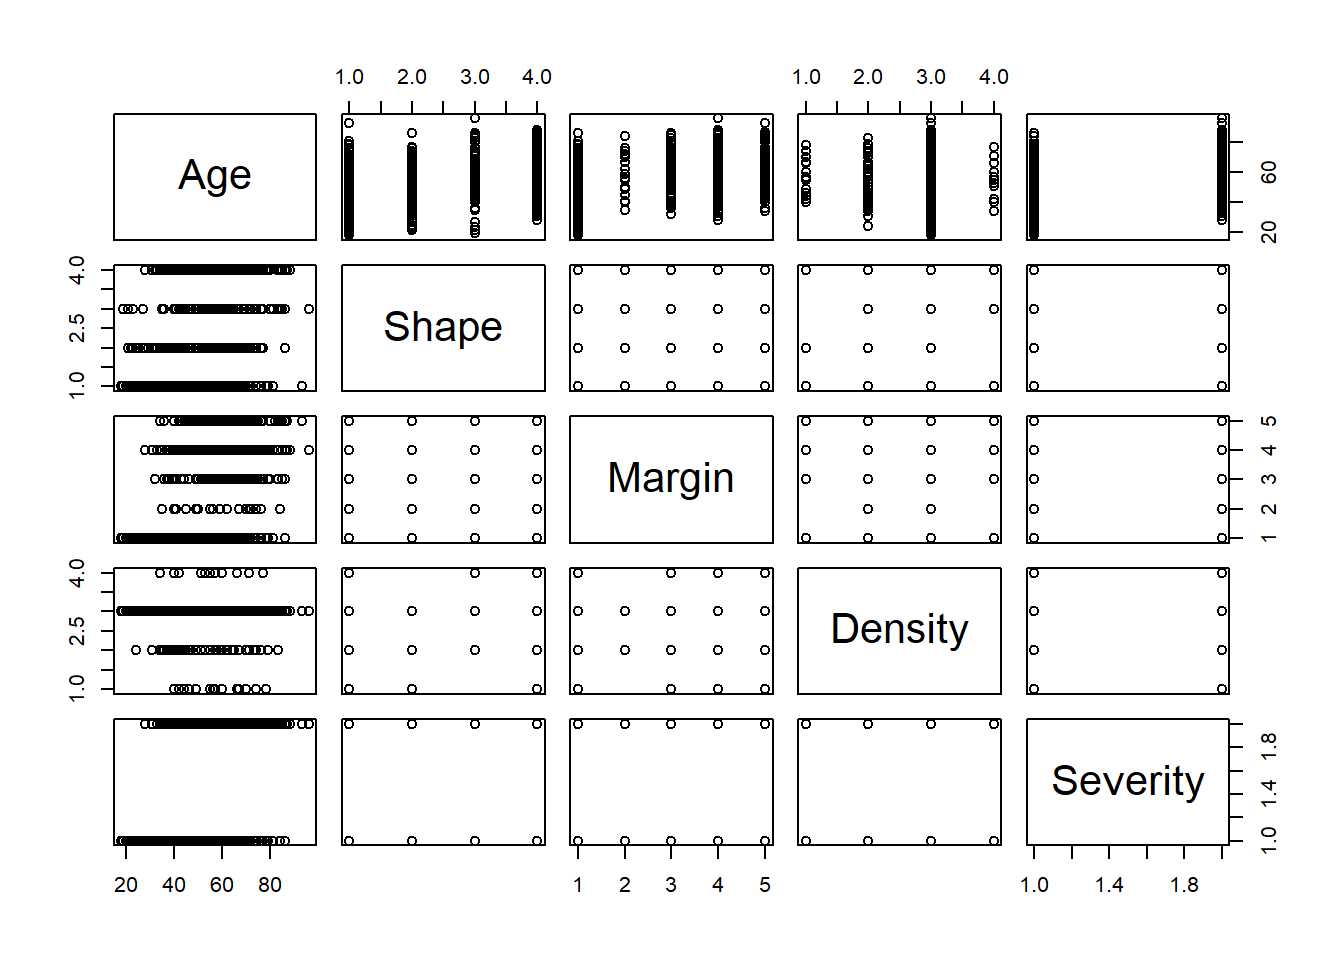
\includegraphics{project_files/figure-latex/unnamed-chunk-25-1.pdf}
\caption{Pairwise scatterplot of Mammographic Mass Severity Data}
\end{figure}

There appears to be a weak,possibly linear, positive relationship
between Age and Severity. There are no observable relationships between
Severity and the other predictors.

\subsection{Model Fitting and Model
Selection}\label{model-fitting-and-model-selection}

We now fit a logistic linear model (M1) to the data, with Severity as
the response variable, and Age, Shape, Margin and Density as the
predictor variables:

\begin{Shaded}
\begin{Highlighting}[]
\NormalTok{full.glm <-}\StringTok{ }\KeywordTok{glm}\NormalTok{(Severity }\OperatorTok{~}\StringTok{ }\NormalTok{Age}\OperatorTok{+}\NormalTok{Shape}\OperatorTok{+}\NormalTok{Margin}\OperatorTok{+}\NormalTok{Density, }\DataTypeTok{data =}\NormalTok{ mammo, }\DataTypeTok{family =} \StringTok{"binomial"}\NormalTok{)}
\KeywordTok{summary}\NormalTok{(full.glm)}
\end{Highlighting}
\end{Shaded}

\begin{verbatim}
## 
## Call:
## glm(formula = Severity ~ Age + Shape + Margin + Density, family = "binomial", 
##     data = mammo)
## 
## Deviance Residuals: 
##     Min       1Q   Median       3Q      Max  
## -2.5286  -0.5632  -0.2190   0.6645   2.5553  
## 
## Coefficients:
##              Estimate Std. Error z value Pr(>|z|)    
## (Intercept) -4.175195   0.847993  -4.924 8.50e-07 ***
## Age          0.054783   0.007807   7.017 2.27e-12 ***
## Shape2      -0.259327   0.319292  -0.812 0.416681    
## Shape3       0.658338   0.375749   1.752 0.079762 .  
## Shape4       1.370209   0.333060   4.114 3.89e-05 ***
## Margin2      1.640629   0.559287   2.933 0.003352 ** 
## Margin3      1.182762   0.351871   3.361 0.000776 ***
## Margin4      1.483740   0.302603   4.903 9.43e-07 ***
## Margin5      2.012203   0.374699   5.370 7.87e-08 ***
## Density2    -0.959989   0.797154  -1.204 0.228485    
## Density3    -0.653906   0.718090  -0.911 0.362497    
## Density4    -1.751671   1.062852  -1.648 0.099335 .  
## ---
## Signif. codes:  0 '***' 0.001 '**' 0.01 '*' 0.05 '.' 0.1 ' ' 1
## 
## (Dispersion parameter for binomial family taken to be 1)
## 
##     Null deviance: 1151.26  on 830  degrees of freedom
## Residual deviance:  726.96  on 819  degrees of freedom
##   (130 observations deleted due to missingness)
## AIC: 750.96
## 
## Number of Fisher Scoring iterations: 5
\end{verbatim}

The p-values for all levels of Density are above 0.05, indicating that
it is not statistically significant at the 0.05 level. This suggests
that removing Density may lead to a more parsimonious model. We first
construct the model without Density (asm.glm).

\begin{Shaded}
\begin{Highlighting}[]
\NormalTok{asm.glm <-}\StringTok{ }\KeywordTok{glm}\NormalTok{(Severity }\OperatorTok{~}\StringTok{ }\NormalTok{Age}\OperatorTok{+}\NormalTok{Shape}\OperatorTok{+}\NormalTok{Margin, }\DataTypeTok{data =}\NormalTok{ mammo, }\DataTypeTok{family =} \StringTok{"binomial"}\NormalTok{)}
\KeywordTok{summary}\NormalTok{(asm.glm)}
\end{Highlighting}
\end{Shaded}

\begin{verbatim}
## 
## Call:
## glm(formula = Severity ~ Age + Shape + Margin, family = "binomial", 
##     data = mammo)
## 
## Deviance Residuals: 
##     Min       1Q   Median       3Q      Max  
## -2.5004  -0.5514  -0.2399   0.6651   2.5963  
## 
## Coefficients:
##              Estimate Std. Error z value Pr(>|z|)    
## (Intercept) -4.719544   0.465771 -10.133  < 2e-16 ***
## Age          0.053879   0.007499   7.185 6.72e-13 ***
## Shape2      -0.447844   0.306327  -1.462 0.143747    
## Shape3       0.499251   0.364446   1.370 0.170721    
## Shape4       1.242837   0.324256   3.833 0.000127 ***
## Margin2      1.582943   0.539614   2.933 0.003352 ** 
## Margin3      1.263073   0.342531   3.687 0.000226 ***
## Margin4      1.543226   0.294045   5.248 1.54e-07 ***
## Margin5      2.032105   0.362892   5.600 2.15e-08 ***
## ---
## Signif. codes:  0 '***' 0.001 '**' 0.01 '*' 0.05 '.' 0.1 ' ' 1
## 
## (Dispersion parameter for binomial family taken to be 1)
## 
##     Null deviance: 1226.93  on 886  degrees of freedom
## Residual deviance:  773.89  on 878  degrees of freedom
##   (74 observations deleted due to missingness)
## AIC: 791.89
## 
## Number of Fisher Scoring iterations: 5
\end{verbatim}


\end{document}
